\section{Architecture for the deployment of a policy matching algorithm for access control}
\label{sec:architecture}

In this Section, a detailed decomposition of the architectural building blocks for a legally-aligned, decentralised personal datastores ecosystem is modelled and documented using the C4 graphical notation model \citep{brown_c4_2015}.
The C4 model is a formalisation used to visualise software architecture, based on the 4+1 View Model of software architecture \citep{kruchten_41_1995}, which has evolved over the years to showcase different views of software components, each of which addresses a specific set of issues, inspired by the Unified Modelling Language (UML).
The main objectives of this model are (i) to simplify the description and understandability of software systems for software developers and (ii) to decrease the gap between source code and software architecture modelling.
The four visualisations of the C4 model have the subsequent goals:

\begin{itemize}
    \item The \textit{System Context} diagram serves as an initial framework for illustrating and documenting a software system, providing an overview that allows for a comprehensive understanding of the system's environment. It typically features the system to be decomposed as a central entity, surrounded by its users and other interconnected systems. The emphasis lies in presenting a broad perspective of the system landscape for non-technical audiences, with less emphasis on intricate details. The primary focus is on identifying people, e.g. users or roles, and software systems, rather than delving into technical specificities such as technologies or protocols.
    \item The \textit{Container} diagram offers an overview of the software architecture's structure at a high level, delineating the allocation of responsibilities within it. Furthermore, it illustrates the primary technological selections and elucidates the communication channels between components, e.g., server-side web applications, mobile apps, or file systems.
    \item The \textit{Component} diagram illustrates the decomposition of a container into various components, elucidating the purpose of each component, and the technological or implementation details involved.
    \item The \textit{Code} diagram is an optional visualisation, recommended only for critical components, that zooms in on each component to illustrate its implementation as code, employing UML class diagrams, entity relationship diagrams, or comparable methods.
\end{itemize}

In the following Sections, the architectural model for a legally-aligned, decentralised personal datastore will be discussed in detail through context, container, and component diagrams.
A special focus will be given to the proposed personal datastore server implementation, and the agreement generator and datastore containers and their components. 

\subsection{System context modelling of a decentralised data sharing ecosystem}
\label{sec:c4_context}

The \textit{System Context} diagram in Figure~\ref{fig:c4-context} illustrates how decentralised personal datastores interact with legal entities and/or natural people and with internal and external software systems at a very high level.
This diagram depicts the decentralised personal datastore server at the centre with no details of its containers, surrounded by all its interacting systems and actors.
The depicted server architecture is aligned with the existing Solid protocol specification \citep{capadisli_solid_2022} and existing CSS and ESS server implementations.

\begin{figure}[ht]
    \centering
    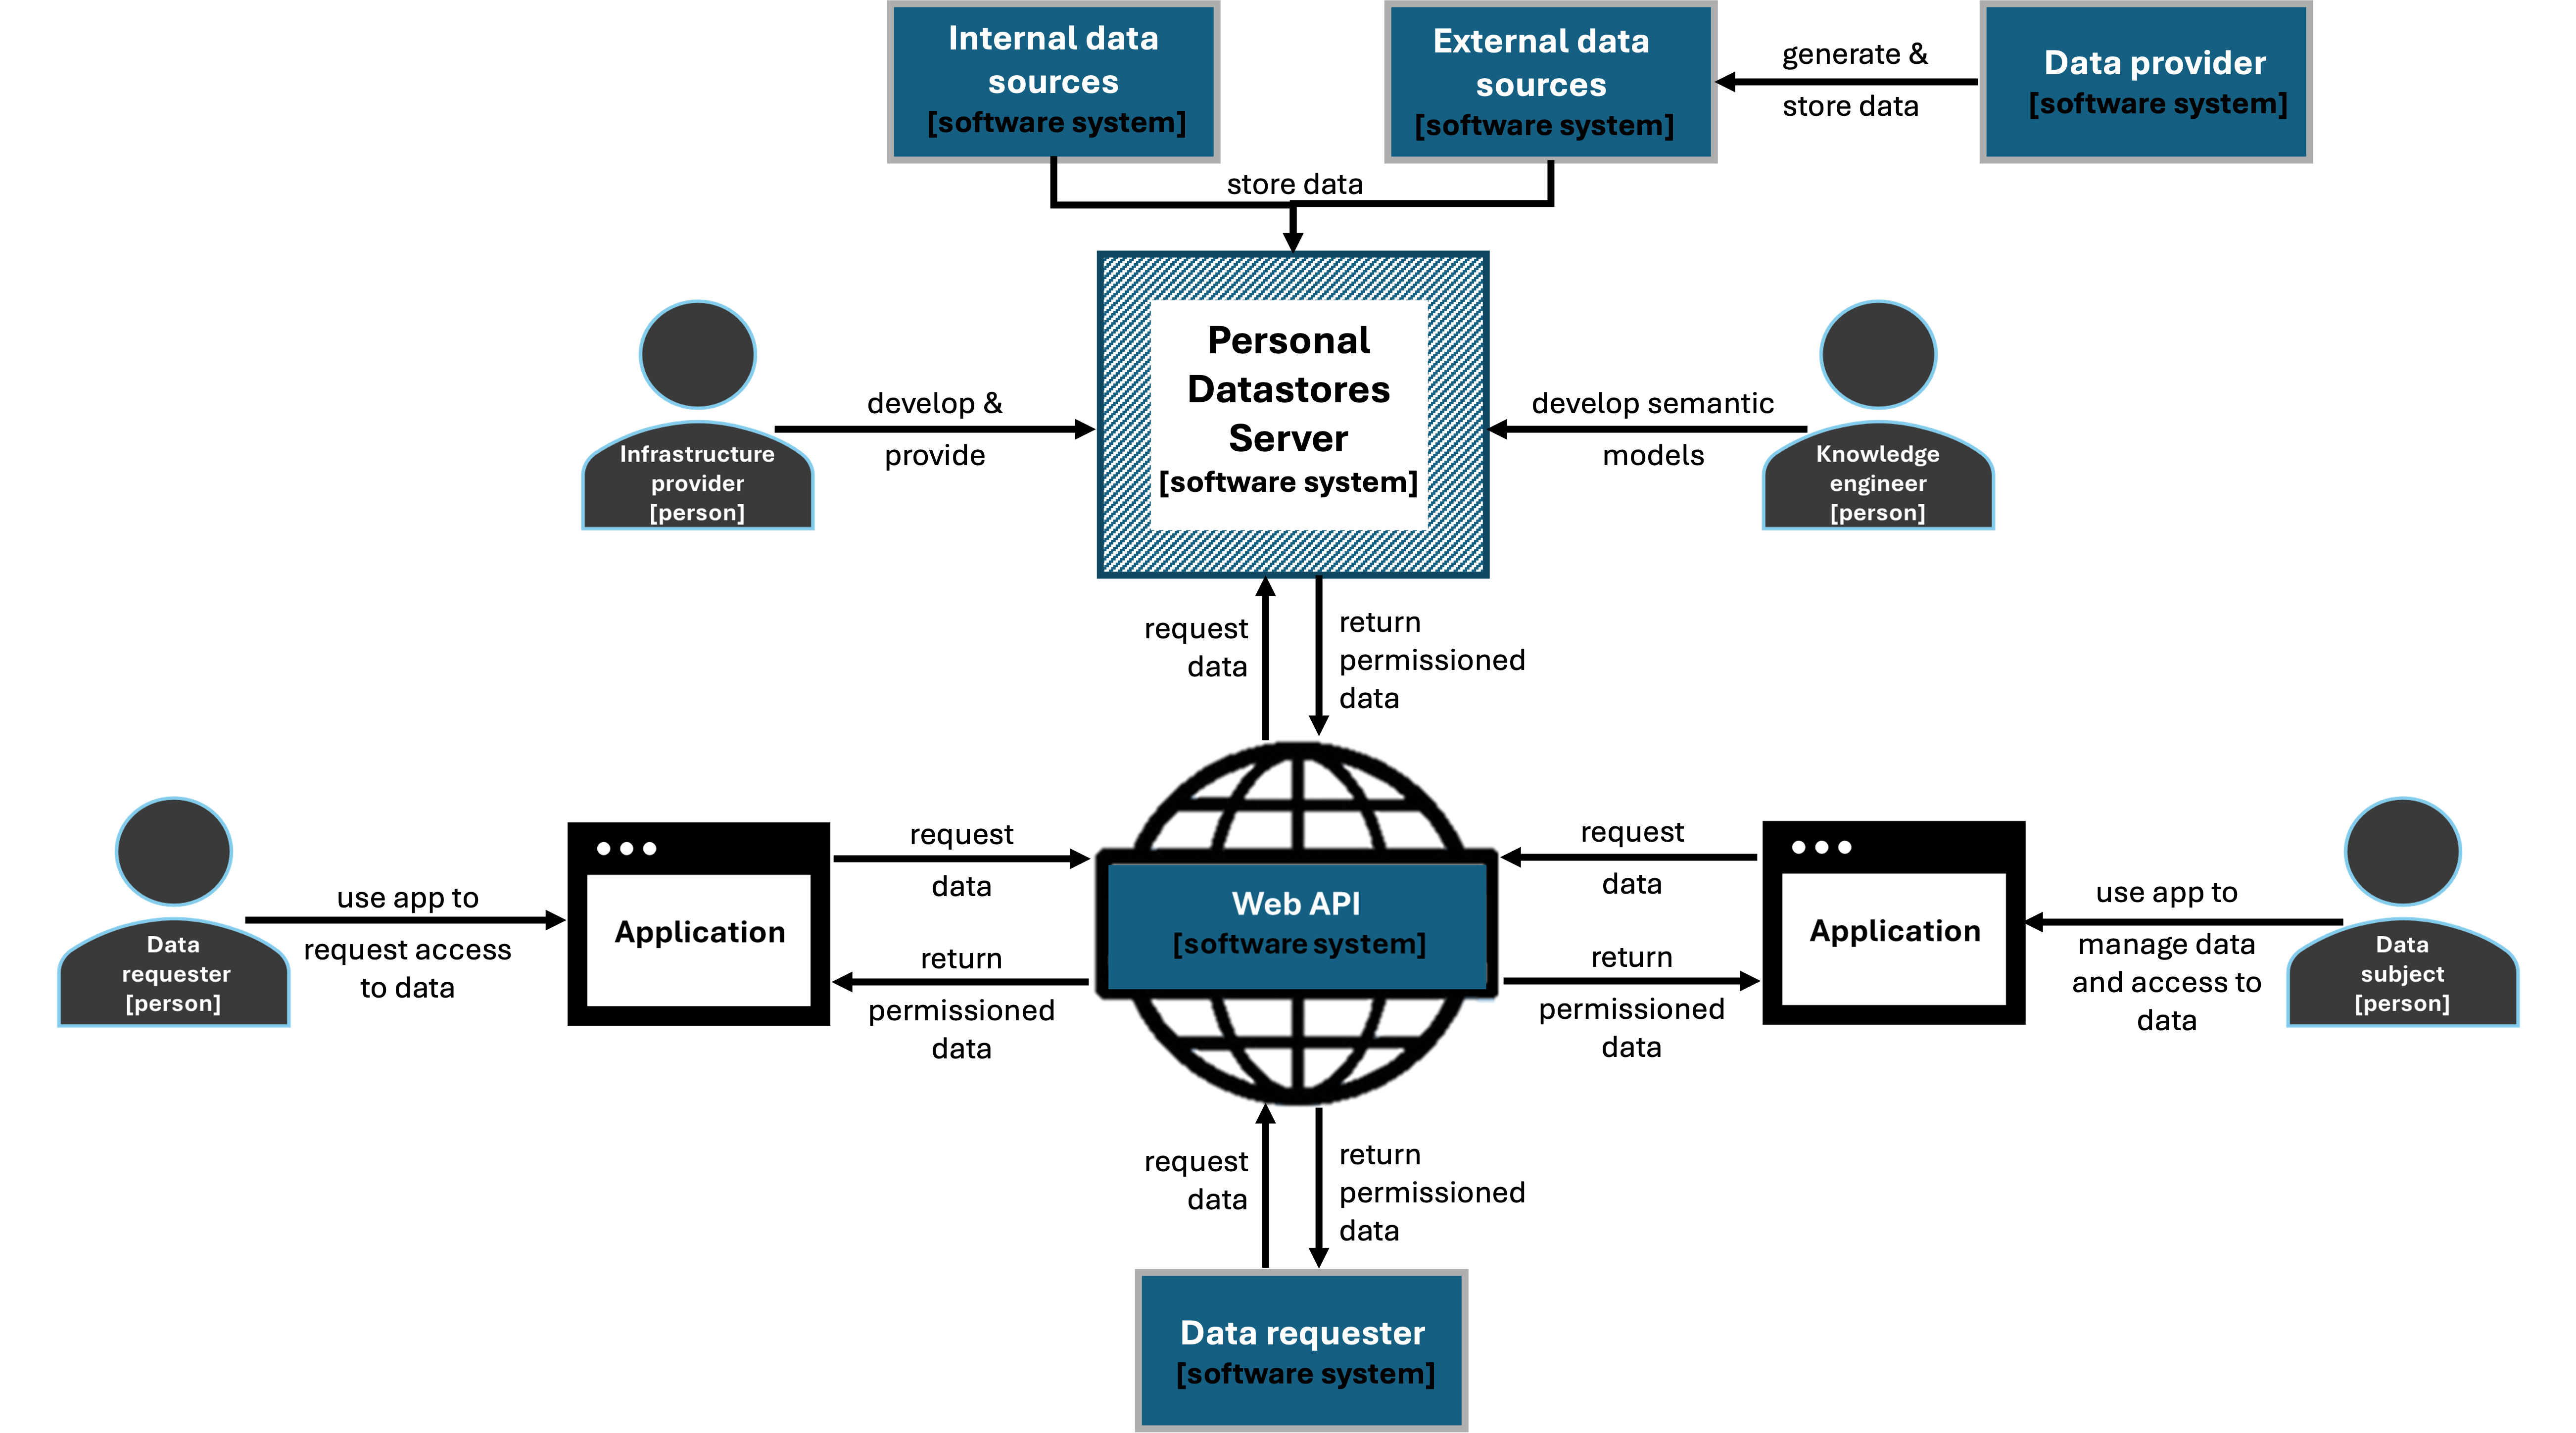
\includegraphics[width=1\linewidth]{figures//chapter-6/system-context-diagram.png}
    \caption{System context diagram of a decentralised data sharing ecosystem.}
    \label{fig:c4-context}
\end{figure}

In this diagram, the \textit{Infrastructure provider} and the \textit{Knowledge engineer} develop and provide services and semantic models for the main software system described in this Section, the \textit{Personal Datastores Server}.
Datastores hosted in this server are populated by internal and external data sources, such as temporal and spatial data sources, respectively.
The server also provides the access control layer of the ecosystem, allowing data requests and the return of permissioned data to be consumed by Web APIs.
Such APIs can be used by \textit{Data requesters} to consume and generate data, and also to feed Web applications that are used by individuals to request and use data.
Moreover, data subjects can also use applications to manage their data and who/what can have access to it under which conditions.

The \textit{Personal Datastores Server} depicted in this Figure will be further decomposed into containers in the next Section.

\subsection{Container modelling of a decentralised personal datastore server}
\label{sec:c4_container}

The \textit{Container} diagram in Figure~\ref{fig:c4-container} illustrates current and proposed containers within a decentralised personal datastores server.
In a completely decentralised scenario, each container could be developed and/or provided by a distinct \textit{Infrastructure provider}.
The \textit{Notifications}, \textit{Authentication} and \textit{Authorisation} containers are already part of the Solid protocol specification \citep{capadisli_solid_2022} and are not further updated in this Thesis.
To ensure compatibility with the current access control mechanisms, the \textit{Offer Instantiation} and \textit{Agreement Generator} containers are treated separately from the \textit{Authorisation} container.
In this way, systems that currently rely on WAC or ACP to provide access to data can continue to work efficiently, while use cases that involve personal data can use OAC policies to have data access agreements aligned with European data protection law.
ACL and ACP authorisations can be generated, when an agreement for data access has already been reached, for automated access to data when a legally-aligned agreement for access is already in place.
The \textit{Notifications} container can also be updated to support the new access control system proposed in this Thesis, however, this is out of the scope of this contribution.

\begin{figure}[ht]
    \centering
    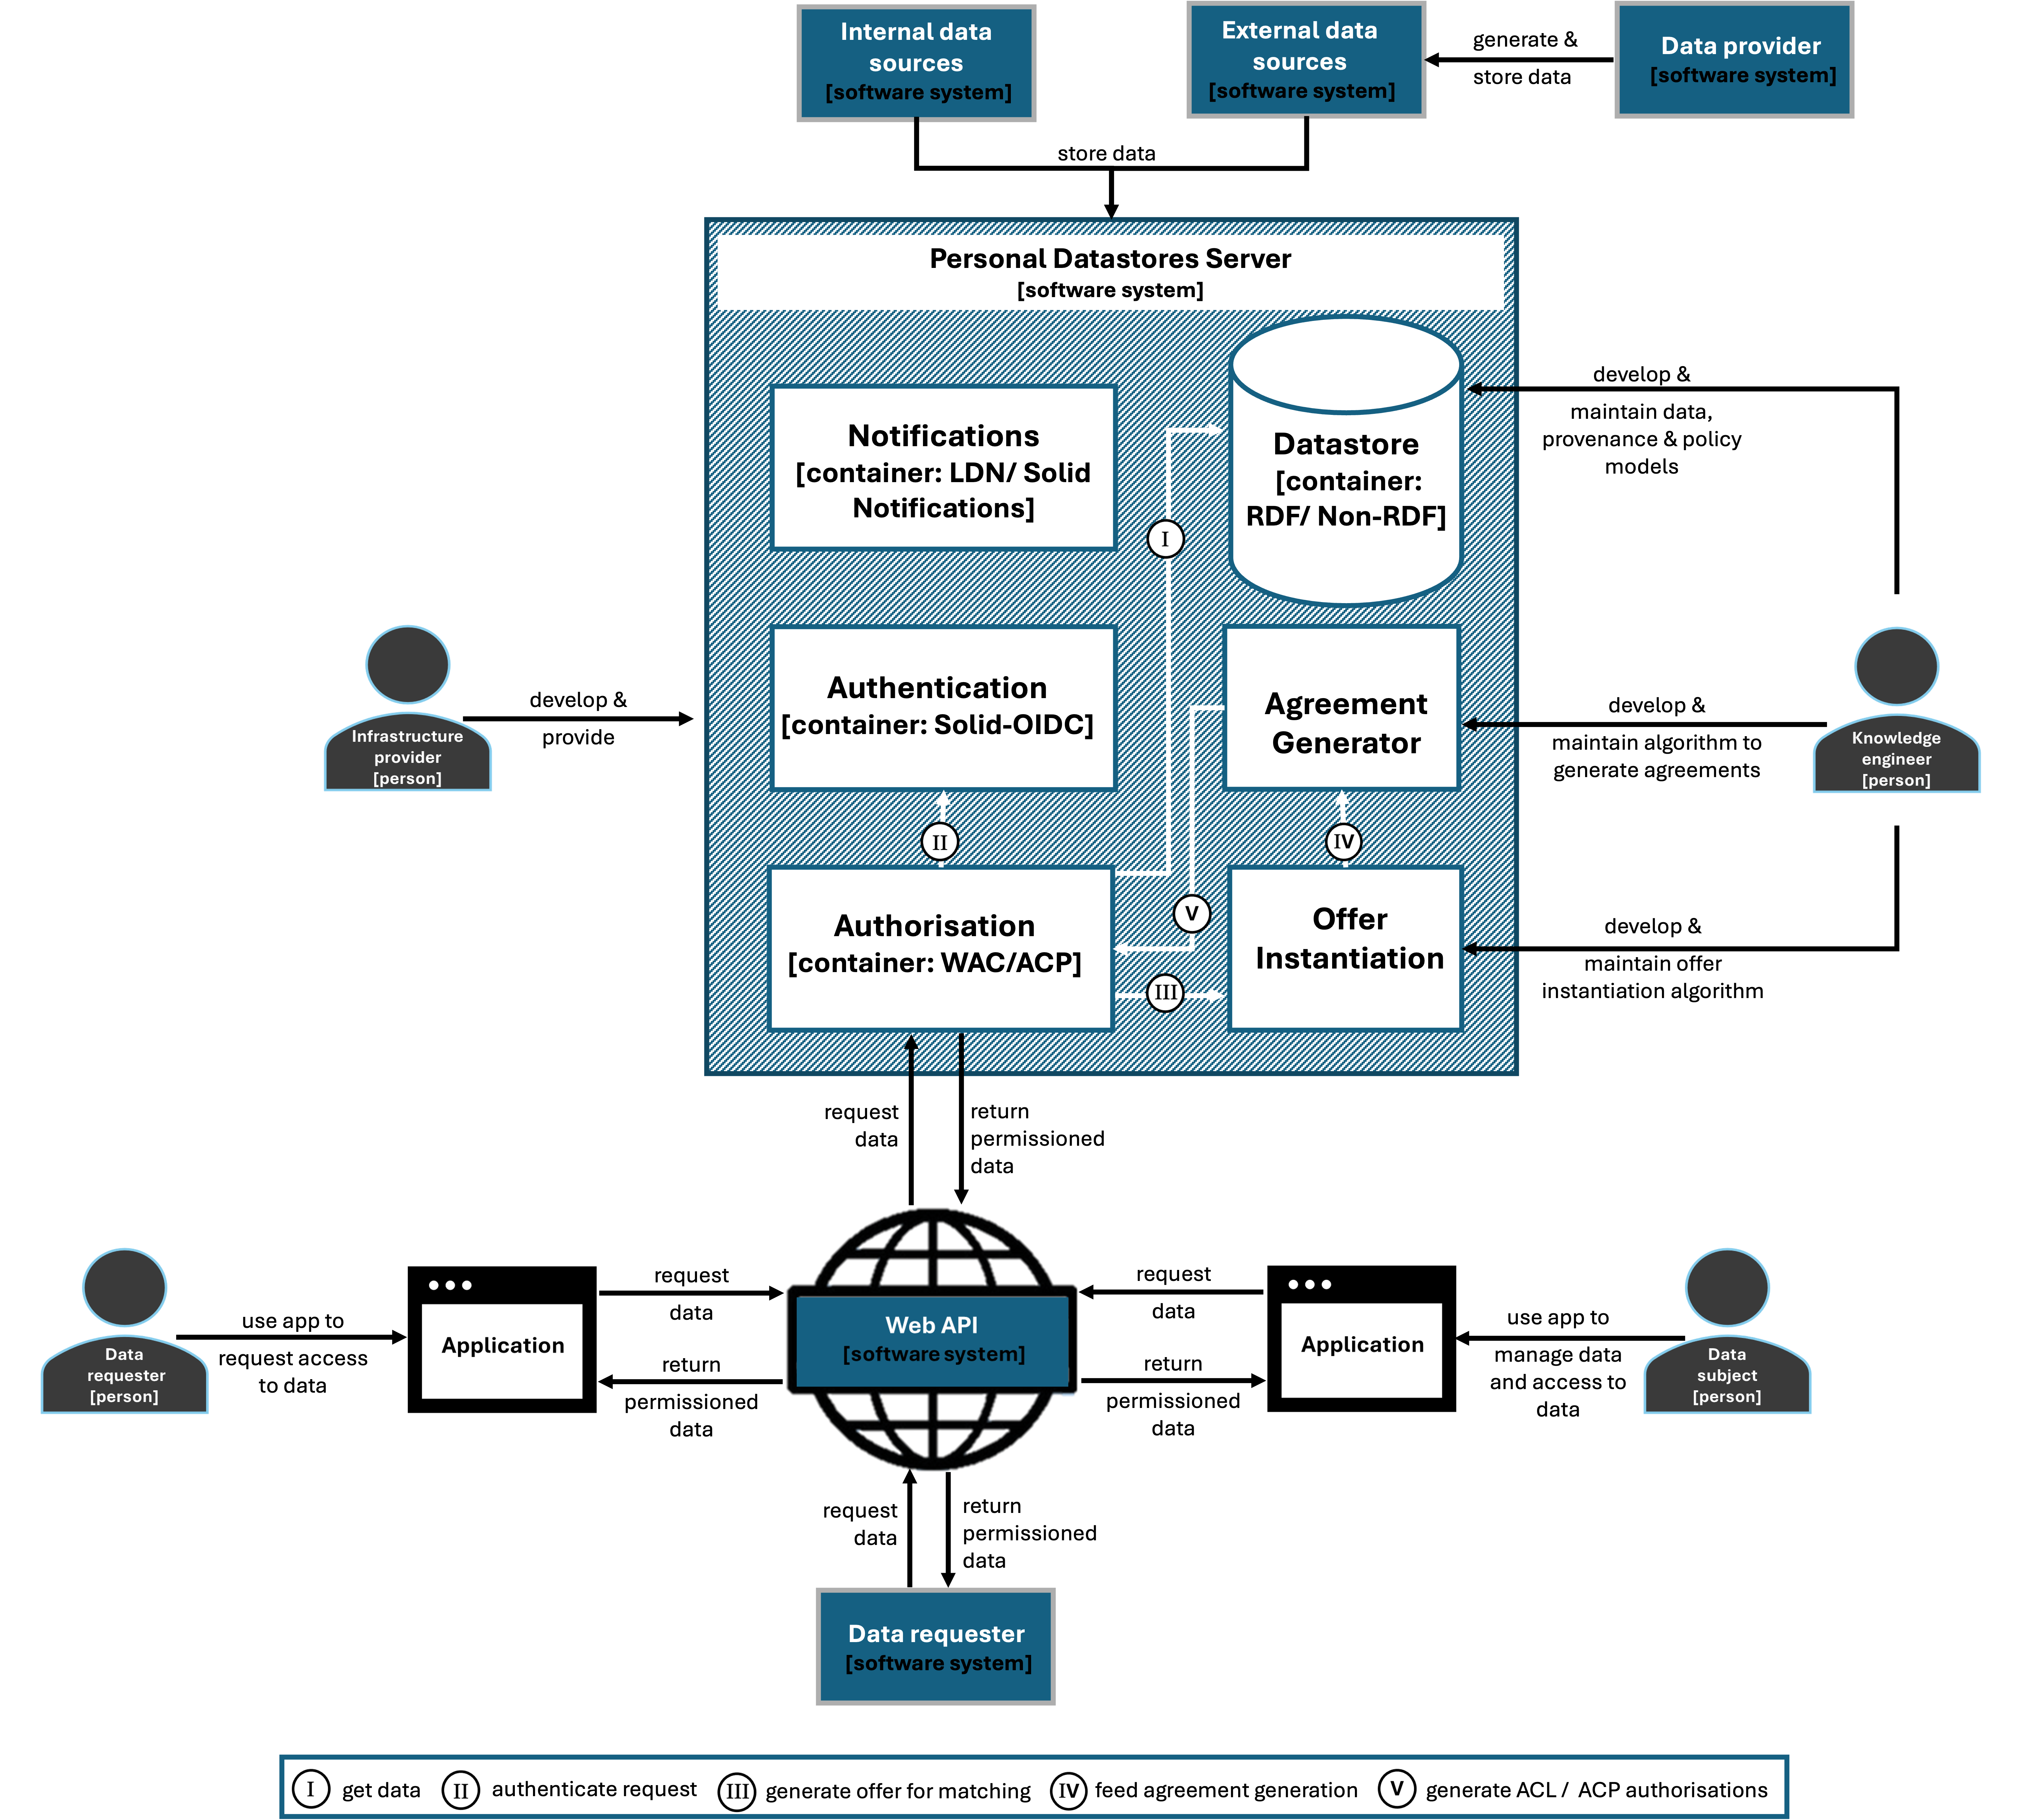
\includegraphics[width=1\linewidth]{figures//chapter-6/container.png}
    \caption{Container diagram of a decentralised personal datastore server.}
    \label{fig:c4-container}
\end{figure}

Furthermore, while an intricate part of the Solid protocol already, the \textit{Datastore} container is further expanded in this Thesis with additional components related to policies and provenance metadata.
The vocabularies developed in Chapter~\ref{chap:vocabularies} should be further developed and maintained by a \textit{Knowledge engineer} and are used to specify data, provenance, and policies, as well as to feed the \textit{Offer Instantiation} and \textit{Agreement Generator} containers.
The \textit{Offer Instantiation} container gathers and instantiates ODRL offers, such as the one in Listing~\ref{list:oac_offer}, which are fed to the \textit{Agreement Generator} container.
This instantiation process takes the user's preferences and requirements to create a context-appropriate offer policy, i.e., directly applicable to the data request.
While the implementation of an offer instantiation algorithm for specific data requests is not conducted in this Thesis, in Section~\ref{sec:poc_health}, there is a description and implementation of the construction of odrl:Offer instances for a particular use case related to health data-sharing.
The \textit{Agreement Generator} depicted in Figure~\ref{fig:c4-container} will be further decomposed into components in the next Section.

\subsection{Component modelling of a datastore and an agreement generator}
\label{sec:c4_component}

The \textit{Component} diagram in Figure~\ref{fig:c4-component} further decomposes the \textit{Datastore} and \textit{Agreement Generator} containers within a decentralised personal datastores server.
As previously discussed in Sections~\ref{sec:oac} and~\ref{sec:plasma}, for a legally-aligned decentralised ecosystem where personal data is exchanged according to the requirements of the GDPR, information regarding the entities (e.g., providers, developers), infrastructure, legal roles, policies, notices, registries, and logs is necessary to understand and establish responsibilities and accountability within the whole ecosystem.
As such, beyond keeping \textit{Data} in distinct formats, \textit{Datastores} are expected to keep (i) \textit{Policies}, including user requirements and preferences, copies of data requests and records of data access agreements, (ii) \textit{Notices}, e.g., to declare the providers/developers of apps, service, or other infrastructures, as well as to describe their data processing practices, (iii) \textit{Logs}, related to actions on data, policies, or security issues, which can be used by external auditors to perform their duties, (iv) \textit{Registries}, for collective and convenient access to data, and (iv) other \textit{Provenance} metadata, all needed to have a trustful and sustainable decentralised data sharing ecosystem.
As such, the semantic models produced in Chapter~\ref{chap:vocabularies} play an important role in having interoperable datastores where data can be consumed by multiple parties in a lawful manner, even if said parties resort to the use of different providers.

\begin{figure}[t]
    \centering
    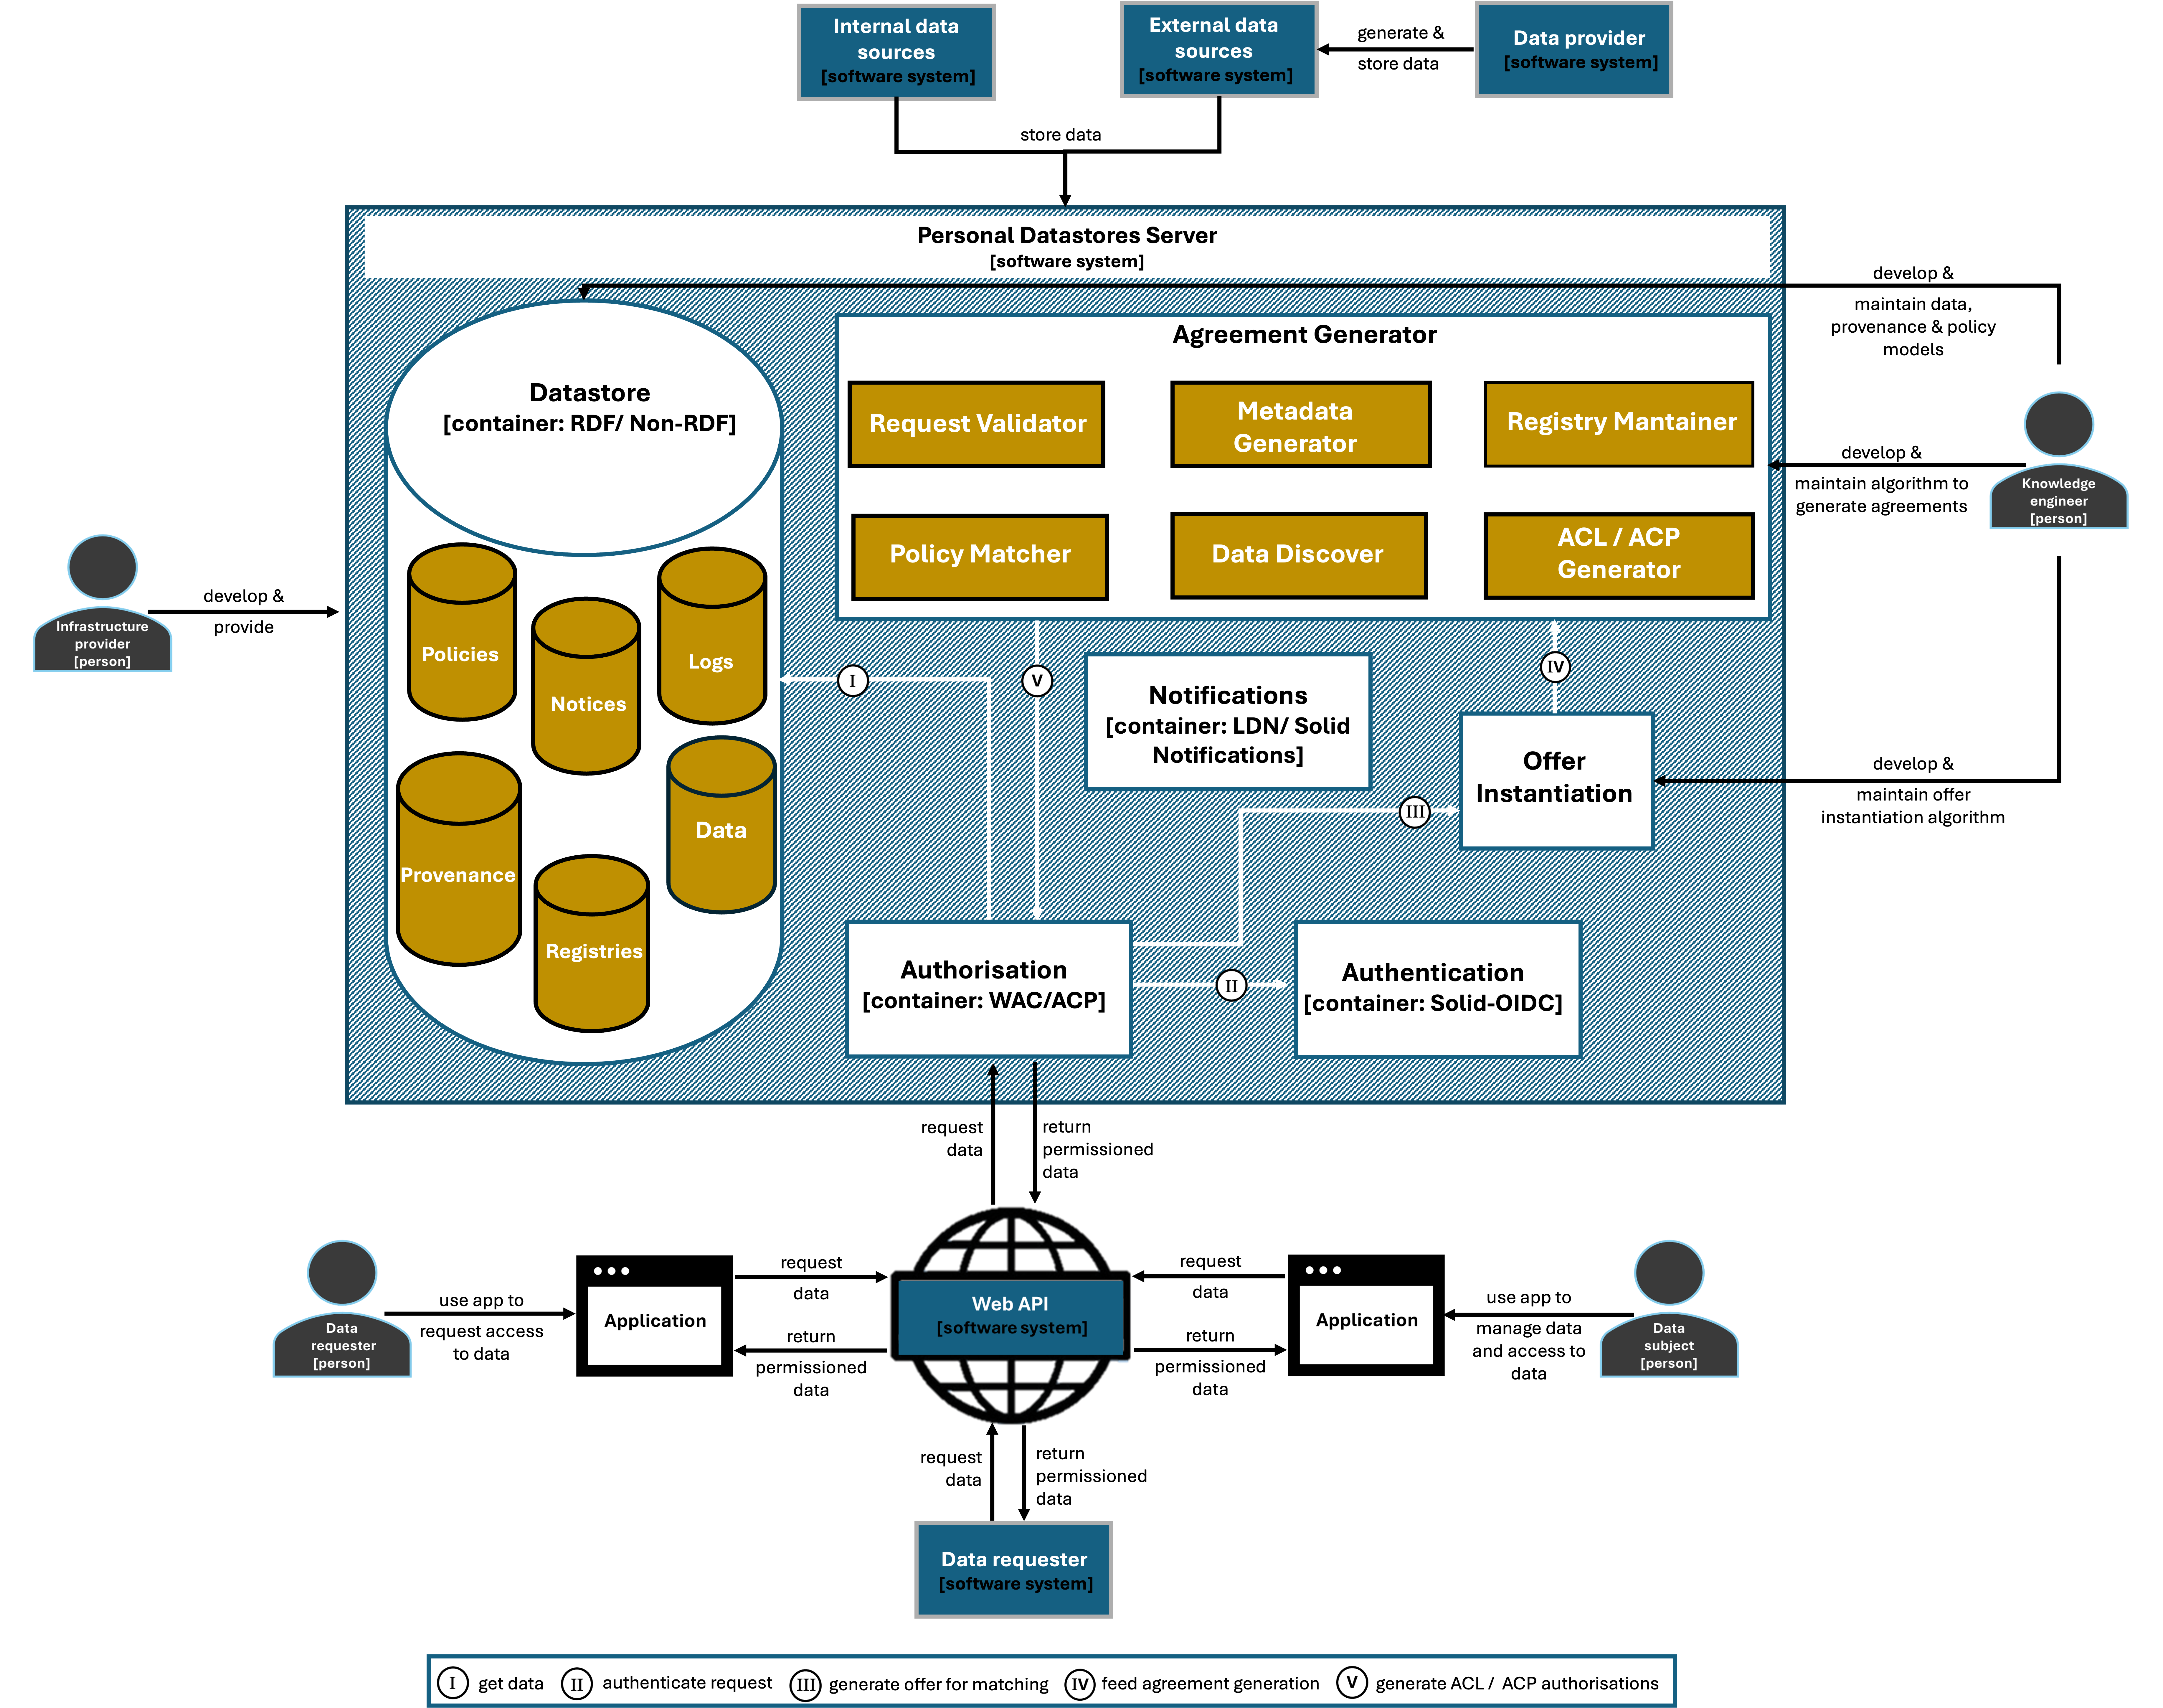
\includegraphics[width=1.1\linewidth]{figures//chapter-6/component.png}
    \caption{Component diagram of a datastore and an agreement generator.}
    \label{fig:c4-component}
\end{figure}

When it comes to the architecture of the \textit{Agreement Generator}, the following components were identified:

% TODO: https://github.com/RDFLib/pySHACL
\begin{itemize}
    \item The \textit{Request Validator} component has the main goal of validating RDF-based data requests against the conformance conditions established in Section~\ref{sec:plasma_conformance}, using technologies such as SHACL~\citep{knublauch_shapes_2017} or ShEx~\citep{prudhommeaux_shape_2019}. This component is of fundamental importance to ensure that all legally required data is present in the data request and to guarantee that the data request can be fed to the policy matcher in the expected format.
    \item The \textit{Metadata Generator} and \textit{Registry Maintainer} components have the main goal of generating and storing logs and other metadata related to entities, apps, services, or Pods and maintaining updated registries of access control authorisations, availability of data categories, supported schemas for data, and relevant policies, apps, services, users, or agents.
    \item The \textit{Data Discover} component's main task is to provide the server with data discovery capabilities in order to more easily find where certain types of data, policies, or provenance metadata are stored, including storage locations outside the server.
    \item The \textit{Policy Matcher} component, further specified in Section~\ref{sec:algorithm}, has the main goal of matching the existing user offers with incoming data requests and generate data access agreements. These agreements are then fed to the \textit{ACL/ACP Generator} component for seamless integration into the current Solid ecosystem.
\end{itemize}

Indeed, to understand the detailed functionality of the proposed personal datastores server, Figure~\ref{fig:c4-sequence} presents a sequence diagram to demonstrate how its containers, and more specifically its components, interact with each other when a data requester uses an app to petition a certain type of data to be used for a particular purpose.

\begin{landscape}
\begin{figure}[htp]
    \centering
    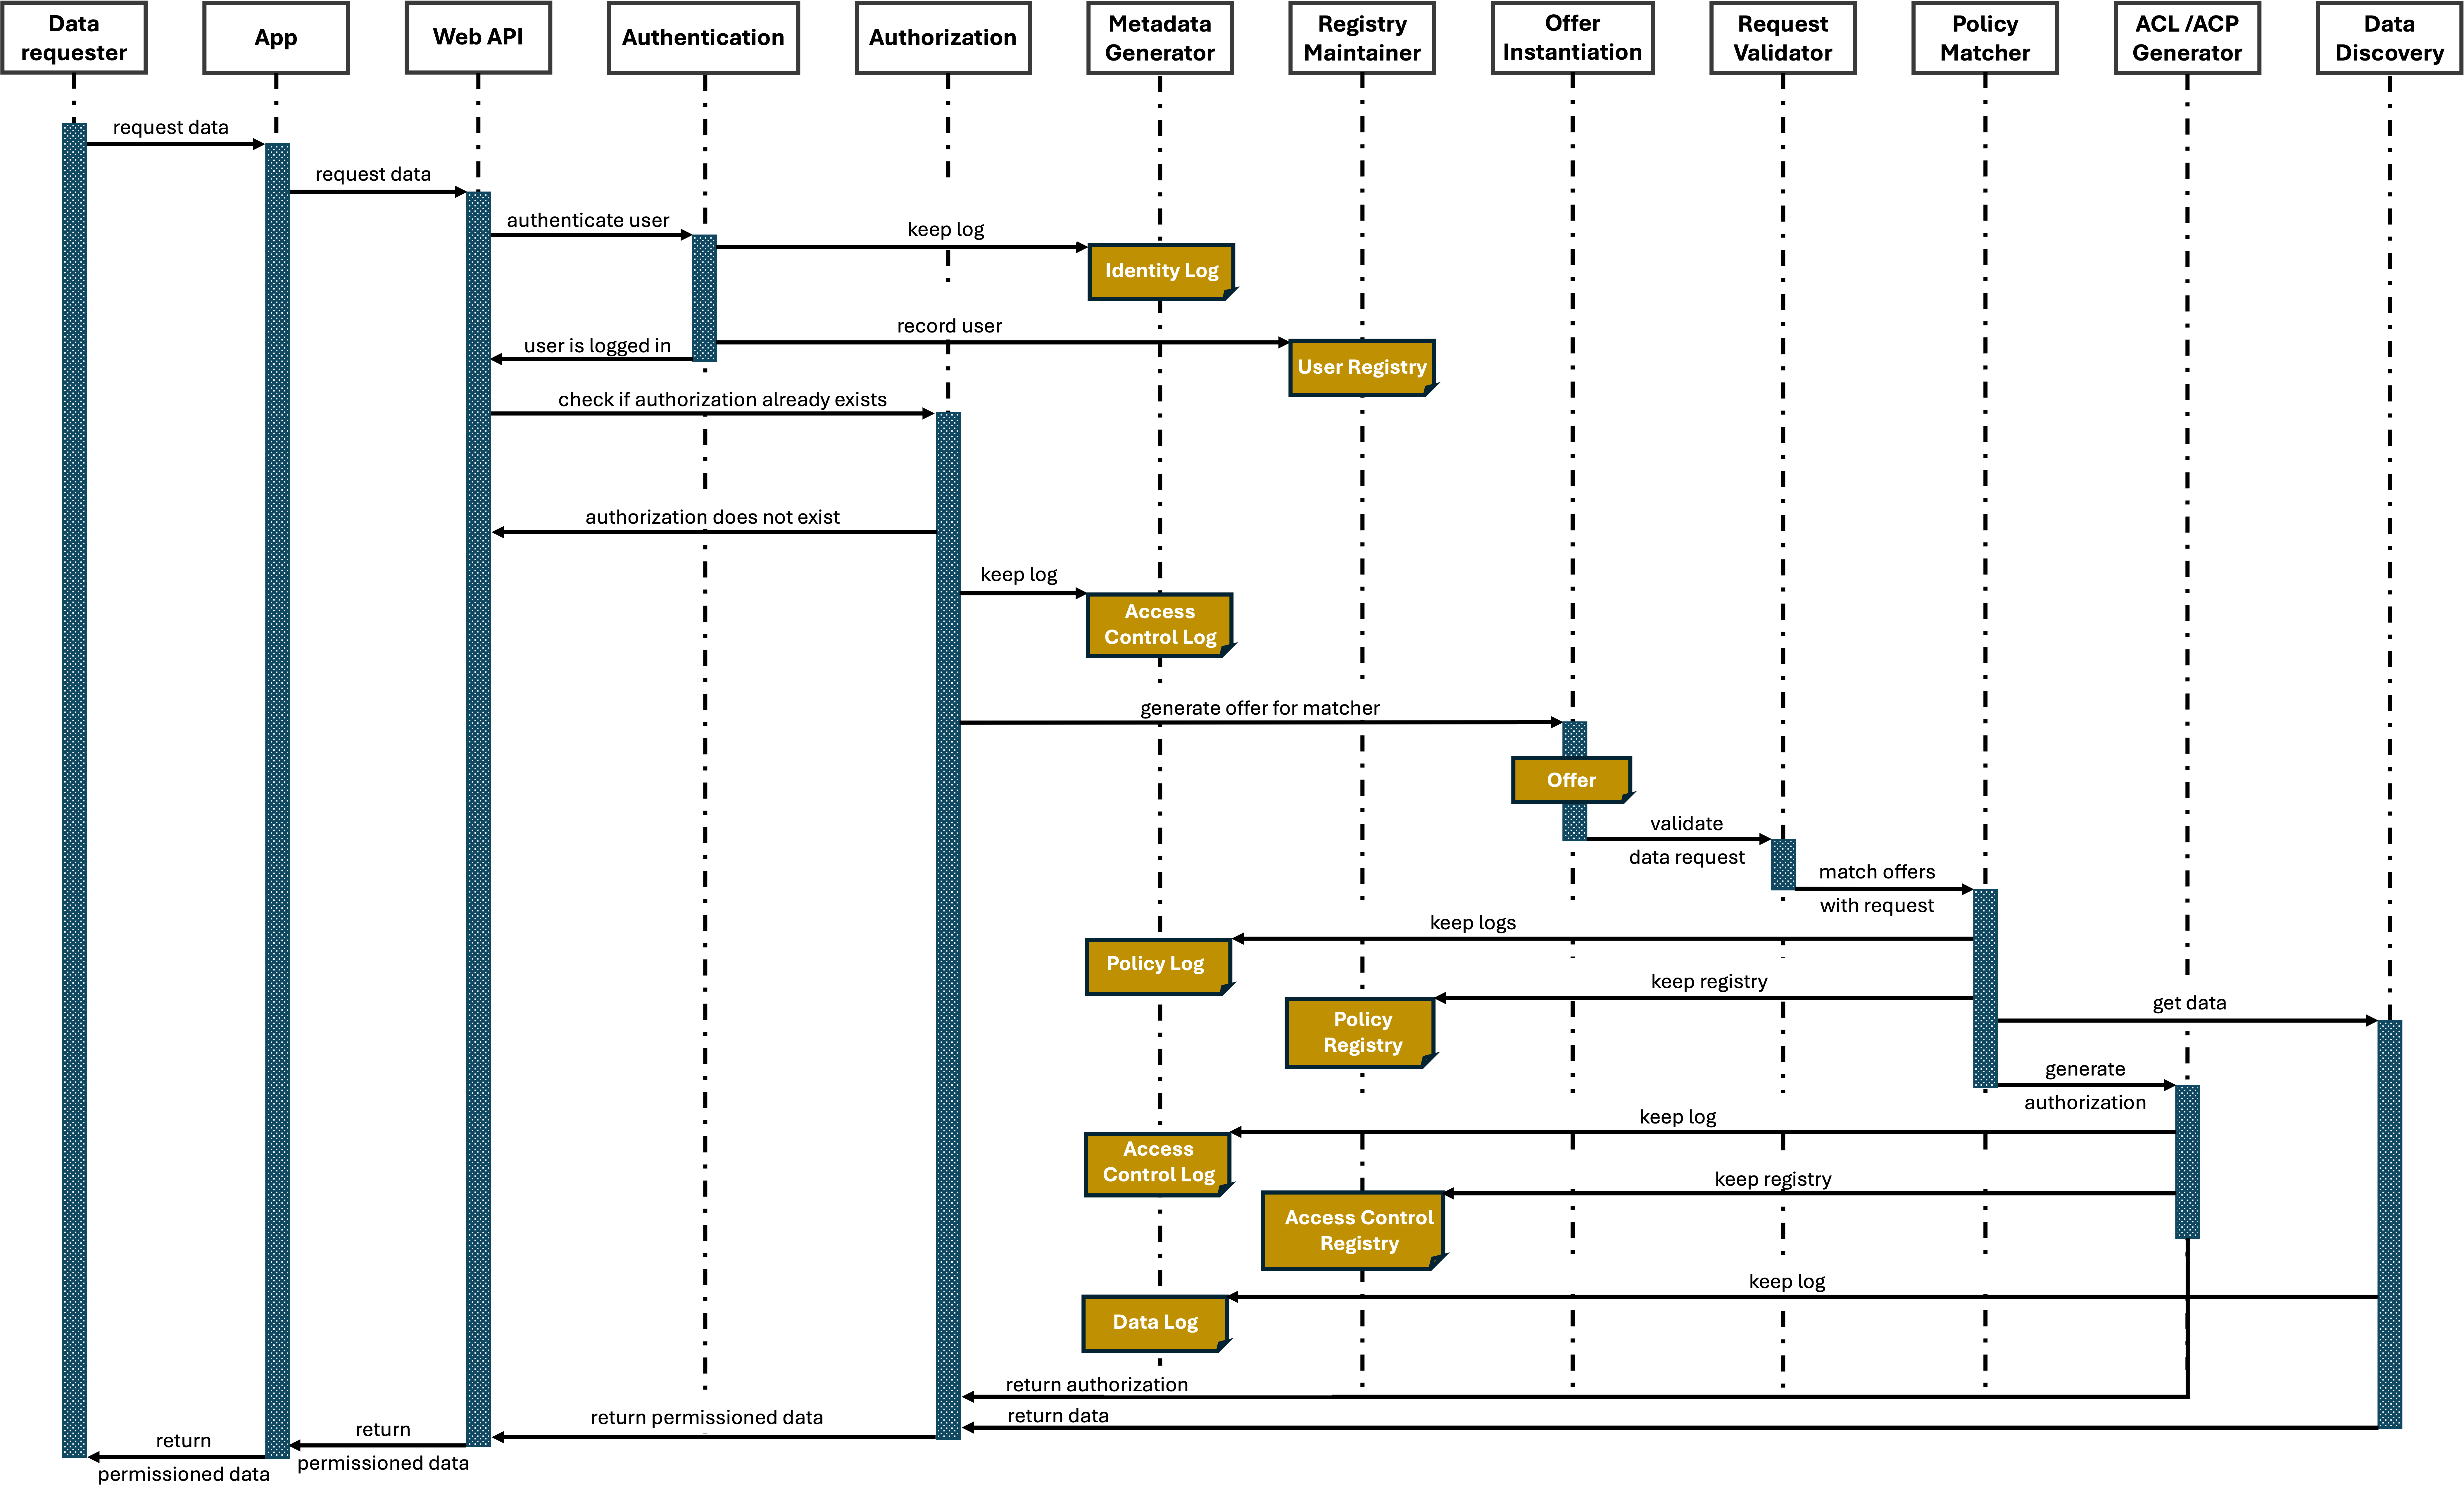
\includegraphics[width=1\linewidth]{figures//chapter-6/sequence.png}
    \caption{Sequence diagram of data access request using proposed architecture.}
    \label{fig:c4-sequence}
\end{figure}
\end{landscape}

When data requesters want to have access to a certain resource or data type, they can either use an app to do it, as in Figure~\ref{fig:c4-sequence}, or directly do a request through the Web API.
When using an app, the request is then transmitted to the Web API and in turn, the requester must be authenticated to get access to non-public data.
After the authentication process goes through, or also in the cases where requesters cannot successfully log in, an identity log is recorded.
Additionally, information about the data requester is also recorded in the user registry of the data subject.
If a previously-given authorisation is still valid, then access to data can be given, however, in Figure~\ref{fig:c4-sequence}, this authorisation does not exist, a fact which could also be kept in an access control log.

Therefore, as there are no ACL nor ACP authorisations in place, an offer with the data subject's policies should be instantiated in order to feed the agreement generator.
This instantiation is followed by the validation of the data request, to ensure that it is in the correct format, and both are fed to the policy matcher component for the generation of a data access agreement.
A log of the policy matching and its result should be kept and the resulting agreement should be added to the policy registry.
In case the result is negative, access to data is prohibited, contrarily to the scenario depicted in Figure~\ref{fig:c4-sequence}.
On the other hand, if the result is positive, access to data is permitted, under certain conditions, and an ACL and/or ACP authorisation is generated.
Afterwards, an access control log is recorded and the new authorisation is kept in the access control log for future usage.
Finally, the data discover mechanism is used to find the data being requested and this data is returned to the Web API and next to the app for the data requester to have access to it.

In the next Section, the algorithms for offer instantiation and for policy matching are further explored, with the goal of generating data access agreements that are aligned with legal requirements.